% !TeX encoding = UTF-8
% !TeX program = xelatex
\documentclass[12pt, a4paper]{article}
\usepackage{xeCJK} % 须放在\usepackage{}列中足够前的位置
\usepackage{fontspec}
\usepackage{graphicx} % 插入圖片
\usepackage{caption}
\usepackage{enumerate}
\usepackage{setspace}
\usepackage{array} % 製作表格必須的宏包
\usepackage{tabularx} % 自動調整列寬的表格宏包
\usepackage{adjustbox}
\usepackage{geometry} 
\usepackage{listings} % 插入程式碼宏包
\setCJKfamilyfont{heiti}{Heiti TC}
\CJKfamily{heiti}
\setmainfont{Arial}
\setstretch{1.5}


\begin{document}
  \begin{center}
    {\Huge 資料結構實習} \\[2.5cm]
    {\Huge Week 02} \\[1.5cm]
    {\Huge 作業報告} \\ [4.5cm]
    \hspace{.6in}
    \begin{minipage}[t]{.4\linewidth}
      {\Large 班級:資訊二甲}\\[0.5cm]
      {\Large 學號:D1109023}\\[0.5cm]
      {\Large 姓名:楊孟憲}
    \end{minipage}    
  \end{center}

  \newpage

  \begin{samepage}
    \fontsize{18pt}{20pt} \selectfont  
    % 生成目錄
    \tableofcontents
    \normalfont
  \end{samepage}
  
  \newpage


  \section{\fontsize{20pt}{22pt}\selectfont 引言}
  \begin{samepage}
    \fontsize{16pt}{18pt} \selectfont
    今天要解的題目是有關於基礎枚舉的方法,以下會討論題目、解題思路、解法說明以及作業心得來做說明。
  \end{samepage}

  % 第一個章節


  \section{\fontsize{20pt}{22pt}\selectfont 題目敘述}
  \begin{samepage}
    \fontsize{16pt}{18pt} \selectfont
    題意說明:撰寫一個程式,輸出 0 和 1 的所有排列變化。\\
    程式說明:輸入一個數字 X,輸出 X 個 bits 所有 0 和 1 的變化。\\
    程式畫面:輸入 4 \\
    \begin{figure}[ht]
      \centering
      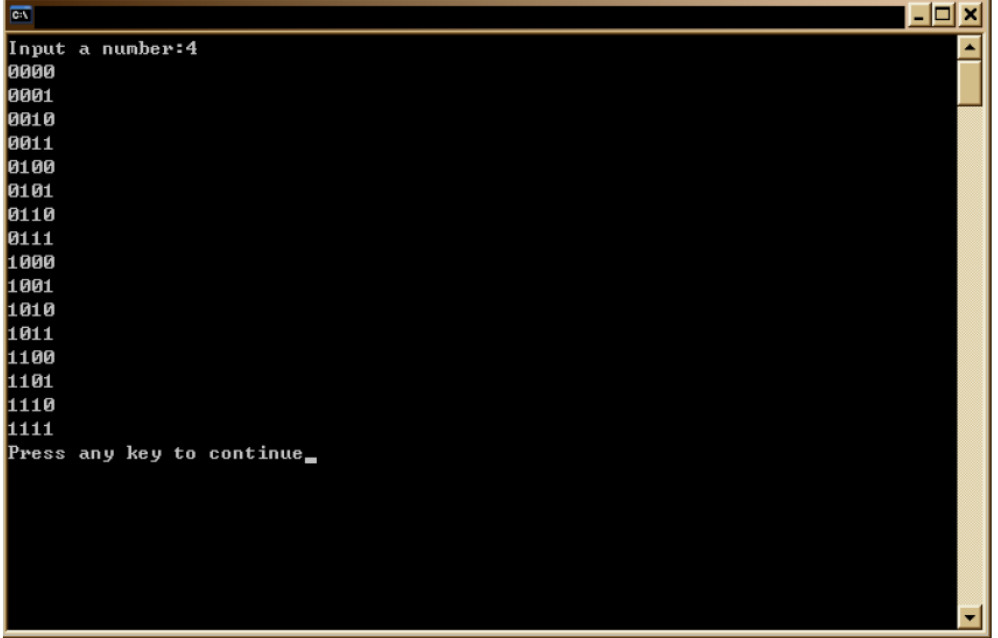
\includegraphics[width=1.0\textwidth]{../image/question.png}
      \caption{執行畫面}
    \end{figure}  
  \end{samepage}
  % 第二個章節

  \section{\fontsize{20pt}{22pt}\selectfont 解題思路}
  % 第二章節的子章節
  \begin{samepage}
    \fontsize{16pt}{18pt} \selectfont
    在這個題目中,輸入$n$,遍歷$n$ 個位元$(0, 1)$的不同的排列組合。在這裡很明顯可以使用 dfs 來實作,是一個深度為 $n$ 時間複雜度為 $O(2^{n})$ 的枚舉。
    \normalfont
  \end{samepage}

  \section{\fontsize{20pt}{22pt}\selectfont 執行結果}
  % 第三個章節
    \begin{samepage}
      \fontsize{16pt}{18pt} \selectfont    
        輸入 4 ,輸出結果:
        \begin{figure}[ht]
          \centering
          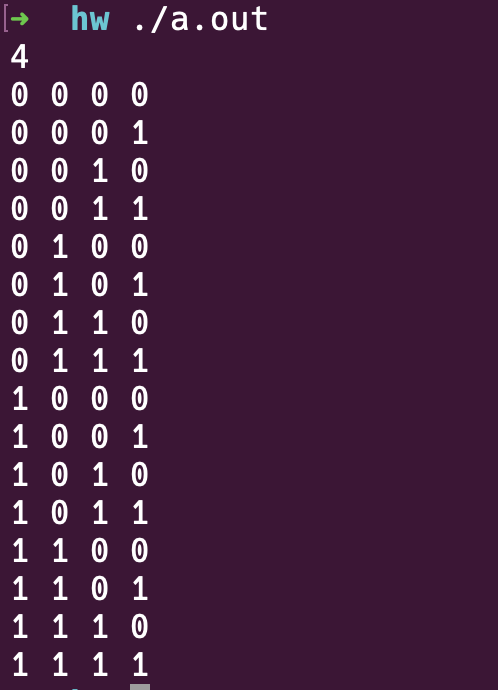
\includegraphics[width=0.6\textwidth]{../image/result.png}
          \caption{執行結果}
        \end{figure}  
      \normalsize
    \end{samepage}

  \section{\fontsize{20pt}{22pt}\selectfont 心得與討論}
  \begin{samepage}
    \fontsize{16pt}{18pt} \selectfont
      這週作業我使用 C++ 實作 dfs,使用 vector 儲存當前答案,實作起來會簡單許多也比較直觀。
      同樣的題目也可以使用位元枚舉來實作 ($000 \to 111$)。我覺得資料結構這門課程可以讓我能更加掌握程式的熟悉度。
    \normalfont
  \end{samepage}
  % 最後一個章節
\end{document}
